\documentclass[sigconf]{acmart}

\usepackage{amsfonts}
\usepackage{enumitem}
\usepackage{svg}
\usepackage{listings}
\usepackage{framed}

\definecolor{blue}{RGB}{37, 70, 100}
\definecolor{red}{RGB}{195, 43, 43}
\definecolor{purple}{RGB}{138, 64, 146}
\definecolor{shadecolor}{RGB}{240, 240, 240}

\lstdefinestyle{mystyle}{
    keywordstyle=\color{red},
    numberstyle=\color{blue},
    stringstyle=\color{purple},
    basicstyle=\ttfamily\small,
    breakatwhitespace=false,
    breaklines=true,
    captionpos=b,
    keepspaces=true,
    showspaces=false,
    showstringspaces=false,
    showtabs=false,
    tabsize=2
}
\lstset{style=mystyle}

\copyrightyear{2026}
\acmYear{2026}
\setcopyright{cc}
\setcctype{by}
\acmConference[SESoS '26]{14th IEEE/ACM International Workshop on Software Engineering for Systems-of-Systems and Software Ecosystems}{April 12--18, 2026}{Rio de Janeiro, Brazil}
\acmBooktitle{14th IEEE/ACM International Workshop on Software Engineering for Systems-of-Systems and Software Ecosystems (SESoS '26), April 12--18, 2026, Rio de Janeiro, Brazil}
\acmDOI{10.1145/3786163.3788453}
\acmISBN{979-8-4007-2395-7/2026/04}

\begin{document}

\title{Open Source Software Ecosystem for Cloud Observability: An Overview and Trends}

\author{Gabriel Silva Fontes}
\email{g.fontes@usp.br}
\affiliation{
  \institution{University of São Paulo}
  \city{São Carlos}
  \country{Brazil}
}

\author{Vasilios Andrikopoulos}
\email{v.andrikopoulos@rug.nl}
\affiliation{
  \institution{University of Groningen}
  \city{Groningen}
  \country{The Netherlands}
}

\author{Elisa Yumi Nakagawa}
\email{elisa@icmc.usp.br}
\affiliation{
  \institution{University of São Paulo}
  \city{São Carlos}
  \country{Brazil}
}

\renewcommand{\shortauthors}{Fontes et al.}

\begin{abstract}

  \textbf{Context}: With the adoption of cloud computing and the evolution
  of IT and software engineering practices, observability, the ability to
  systematically measure and monitor software systems, becomes a growing
  concern. Cloud computing is very heterogeneous, and thus creating,
  maintaining, and observing systems built on it requires integration of
  multiple tools. Open source software (OSS) tooling emerged as a de-facto
  standard in multiple areas, including cloud observability. The ecosystem
  formed by OSS observability tooling is large and often difficult to
  navigate.
  %
  \textbf{Objective}: The main goal of this paper is to present
  the OSS Ecosystem formed by cloud computing observability tooling, by
  providing an overview of the main tools and identifying trends on their
  integration.
  %
  \textbf{Method}: We searched the literature for studies on
  cloud observability and used an automated named-entity recognition (NER)
  method to extract candidate observability tools from abstracts. We
  selected the OSS observability tools according to well-defined criteria.
  Following this, we used keyword matching on the tools' source codes,
  revealing integration code, documentation, and other types of relations.
  %
  \textbf{Results}: As a result, we found 45 OSS observability tools and
  derived quantitative measures on their relations to one another. The
  tools serve different roles in observability stacks, with our results
  serving as a proxy measure on how strongly they relate to one another.
  %
  \textbf{Conclusion}: We present an overview of different tools, how
  frequently they appear, their functionality, and a visualization of
  their relations. Some trends are identified, such as the centrality of
  some tools (e.g. \emph{Prometheus}), common stacks (e.g. \emph{ELK},
  \emph{TICK}), and outliers (\emph{Thingspeak}). We discuss topics such
  as measuring relations, standardization, proprietary lock-in, among
  others.

\end{abstract}

\keywords{Open Source Software, Cloud Computing, Observability, Mining Software Repository}

\begin{CCSXML}
<ccs2012>
   <concept>
       <concept_id>10011007.10010940.10010971.10011120.10003100</concept_id>
       <concept_desc>Software and its engineering~Cloud computing</concept_desc>
       <concept_significance>500</concept_significance>
       </concept>
   <concept>
       <concept_id>10002951.10003227.10003233.10003597</concept_id>
       <concept_desc>Information systems~Open source software</concept_desc>
       <concept_significance>500</concept_significance>
       </concept>
   <concept>
       <concept_id>10002944.10011123.10010577</concept_id>
       <concept_desc>General and reference~Reliability</concept_desc>
       <concept_significance>300</concept_significance>
       </concept>
   <concept>
       <concept_id>10002944.10011123.10011124</concept_id>
       <concept_desc>General and reference~Metrics</concept_desc>
       <concept_significance>300</concept_significance>
       </concept>
 </ccs2012>
\end{CCSXML}

\ccsdesc[500]{Software and its engineering~Cloud computing}
\ccsdesc[500]{Information systems~Open source software}
\ccsdesc[300]{General and reference~Reliability}
\ccsdesc[300]{General and reference~Metrics}

\maketitle

\section{Introduction}\label{introduction}

Catalyzed by the revolution brought by the public cloud and the advance
of modern IT practices, such as the Site Reliability Engineering concept
\cite{beyer2016site} and the DevOps movement, systems administration
is shifting from operational into an engineering domain
\cite{beyer2016site}. With this shift, a need to systematically
measure and monitor software systems emerge that is known as
\emph{observability}. Observability is a concept originating from
control theory, meant to measure the degree to which a system's internal
state can be inferred from its output at any point in time
\cite{niedermaier2019observability}. Cloud observability, in turn,
is the degree to which (cloud) infrastructure, applications deployed on
this infrastructure, and their interactions can be monitored using data
such as logs, metrics, and traces \cite{picoreti2018multilevel}.

The cloud computing ecosystem is, by its very nature, a heterogeneous
combination of different platforms, software, and systems. Ranging from
on-premises infrastructure and traditional workloads, to a multitude of
different cloud providers and cloud-native container orchestration, plus
dozens of different configuration management tools (with varying degrees
of compatibility), the list goes on and on. In this scenario, it is
challenging to create, maintain, and observe systems that rely on such a
diverse ecosystem. This diversity makes the interoperability requirement
critical \cite{6133225} \cite{6480040}. Open Source Software
(OSS) is a natural fit for this, due its effect on standardization and
commodification \cite{Linden2009}. There are many cases where an
OSS' potential for interoperability helped it become a dominant force in
software engineering tooling, including Docker/OCI, Kubernetes, Linux,
Git, LSP, among others. Cloud observability is no different, as we will
discuss further in this work.

Just as the cloud systems that it aims to observe, the OSS ecosystem for cloud
observability is similarly diverse and heterogeneous. This ecosystem includes
tools for tracing, benchmarking, logging, aggregation, storage, visualizations,
alerting \cite{beyer2016site}, with many different tools being combined to
create \emph{observability stacks} that are used in different contexts and
business domains. Understanding this ecosystem becomes crucial for both
researchers in the cloud computing domain, as well as practitioners looking
to build more reliable and observable cloud-based systems. This understanding,
however, is not just about which tools there are out there, but how they
integrate and which role they play in an observability stack.

While there is some non-academic effort to better understand subsets of
this ecosystem \cite{cnf-landscape}, current literature lacks a
wider study on the OSS ecosystem for cloud observability. With that in
mind, the main goal of this paper is to present an overall view of the
OSS tooling ecosystem used for cloud observability. To achieve our goal
and identify trends in this field, we defined two research questions
(RQs):

\begin{itemize}
\item
  \textbf{RQ1}: What are the most relevant OSS tools in cloud
  observability stacks?; and
\item
  \textbf{RQ2}: How are OSS tools combined to form cloud observability
  stacks?
\end{itemize}

Following this, we searched the scientific literature and located 3068 studies,
from which, through an automated extraction followed by manual selection, we
identified 45 OSS observability tools. As a main result, we observed the centrality
of some tools, and tools that cluster together. We intend that the overview
presented in this paper can bring implications for both practitioners and
researchers.

The remainder of this paper is structured as follows:
Section~\ref{research-method} outlines the research method;
Section~\ref{results} reports the main results;
Section~\ref{discussion} presents our main findings, threats to
validity, and future work; Section~\ref{conclusions} concludes
our work.

\section{Research Method}\label{research-method}

Figure~\ref{fig-research-method} provides an overview of the research
method and the reproduction package files that correspond to each step. The
reproduction package is made available both in the supplementary material and
online\footnote{\url{https://github.com/Misterio77/OSS-Cloud-Observability}} to
replicate the entirety of this research.

\begin{figure}[!htbp]
  \centering
  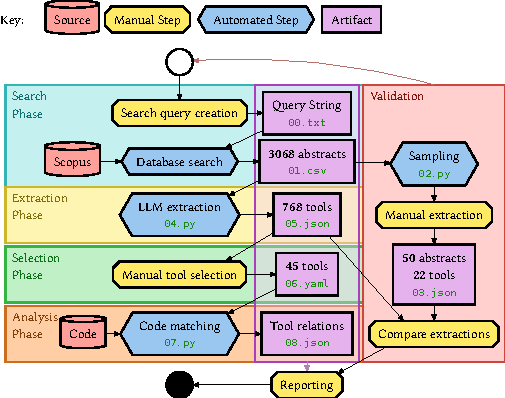
\includegraphics[width=0.90\linewidth]{assets/fig-research-method.pdf}
  \caption{Overview of research method}
  \Description{A flowchart for visualizing the phases and steps for the research method, which are textually explained in the subsections.}
  \label{fig-research-method}
\end{figure}

\subsection{Search Phase}\label{search-phase}

To build our initial set of tools, we used a large population
of research studies as basis. For that, we searched
Scopus\footnote{\url{https://scopus.com}} with the following query:

\begin{snugshade}
\begin{lstlisting}[language=SQL]
  TITLE-ABS-KEY(
    cloud AND tool AND (
      observability OR logging OR monitoring
    )
  ) AND LIMIT-TO(SUBJAREA,"COMP")
\end{lstlisting}
\end{snugshade}

Our goal includes, but is not limited to, finding more niche tools and thus
benefits from a large and diverse sample size. To avoid missing relevant tools,
this search query intentionally did not try to exclude research software nor
proprietary software, thus leaving this filtering for manual selection, as
described in Section~\ref{selection-phase}.

The search resulted in a set of \textbf{3068} studies, which were exported
into a CSV file in the following format: \texttt{"Title",\allowbreak
"Year",\allowbreak "DOI",\allowbreak "Link",\allowbreak "Abstract"}. This
data is available in the reproduction package as \texttt{01\allowbreak
-scopus\allowbreak -search\allowbreak -results\allowbreak .csv}.

\subsection{Extraction Phase}\label{extraction-phase}

This is a problem in the class of Named-entity Recognition (NER)
\cite{pakhale2023ner}, albeit a single-class one. As the intent is to extract
tool names mentioned in the studies, a method that can be aware of context,
such as BERT or an LLM, is ideal. For this extraction, due to ease of access
and previous experience, we decided to use an LLM to extract the tools from
abstracts.

The reason for using the abstracts alone, besides ease of automation and
availability, is that an abstract can fit together with the LLM's prompt
in most models' context windows, drastically reducing hallucinations and
costs when compared to the full texts. The main risk from this strategy
is missing tools that only appear in the full text; hence, we mitigated
it in two ways: (i) by using a large amount of studies; and (ii) by
calibrating the prompt using a validation set, as discussed next.

\subsubsection{Validation sampling and extraction}\label{validation-set}

A validation set of \textbf{50} manually extracted abstracts was created. This
set was used to estimate precision and recall of the overall dataset and to
calibrate the LLM prompt used for extraction. The first attempt was by randomly
sampling abstracts. After analysis, it was evident that the negatives (i.e.,
abstracts not containing any observability tool names) made up around 80-90\%
of the corpus, making the data very sparse. To get a set with a higher share
of positives, we decided to use a combination of keyword spotting (by matching
the text with a few known observability tools\footnote{grafana, prometheus,
graphite, opentelemetry, elasticsearch, fluentd, kibana, logstash,   jaeger,
influxdb, ceilometer}) and random sampling. The set is composed of \textbf{42}
studies originating from keyword match and \textbf{8} from random sampling. The
script that reproduces this step is available in the reproduction package as
\texttt{02-\allowbreak validation-\allowbreak set-\allowbreak script.\allowbreak
py}. The authors then manually extracted tools from these abstracts, inserting
the annotations into the dataset, which is available in the reproduction
package as \texttt{03-\allowbreak validation-\allowbreak set-\allowbreak
results.\allowbreak json}. The validation set was used to evaluate and refine
the study, including the search query and LLM prompt, as discussed next.

\subsubsection{LLM extraction}\label{llm-extraction}

The extraction method consists of feeding each study's abstract to an
LLM (in this case, DeepSeek-V3 \cite{deepseekv3}), with the
following prompt:

`` \emph{You will receive a paper abstract that relates to cloud
observability/monitoring/logging/tracing tools. Enumerate all
observability/monitoring/logging/tracing tools mentioned in it. Respond
with the names separated by comma: \texttt{tool1,tool2,tool3}. If there
are no relevant tools, reply with an empty string.} ''

This prompt was the result of several rounds of evaluation and calibration.
By using the LLM to extract tools from the validation set, we achieved recall
\textbf{97\%}, precision \textbf{69\%}, and $F_1$ \textbf{80\%} (66 true
positives, 30 false positives, and only 2 false negatives). The key metric here
is the recall, as this LLM extraction is then used for a manual selection, so
it is crucial that false negatives are minimized, even if this leads to more
false positives.

From the full set, the LLM extracted a total of \textbf{768} candidate
tools, originating from \textbf{774} studies (\textbf{25\%} of
\textbf{3068} total studies). This step can be fully reproduced via the
script \texttt{04-\allowbreak llm-\allowbreak extraction-\allowbreak script.\allowbreak py}, and its results are
available in \texttt{05-\allowbreak llm-\allowbreak extraction-\allowbreak results.\allowbreak json}. These tools were
then manually selected, as detailed in
Section~\ref{selection-phase}.

\subsection{Selection Phase}\label{selection-phase}

We manually examined the 768 candidate tools and the studies they
appeared on and selected the tools according to the following selection
criteria:

\begin{itemize}
\item
  Inclusion Criteria (IC):

  \begin{itemize}
  \item
    \textbf{IC1}: The tool is/was a piece of Free/Open Source Software,
    meaning licensed under one of the OSI\footnote{\url{https://opensource.org/licenses}}'s
    or FSF\footnote{\url{https://gnu.org/licenses/license-list.html}}'s
    approved software licenses; and
  \item
    \textbf{IC2}: The tool is used/discussed as part of a cloud
    observability solution.
  \end{itemize}
\item
  Exclusion Criterion (EC):

  \begin{itemize}
  \item
    \textbf{EC1}: The tool is a piece of research software and not
    otherwise available as an actual FOSS project on the web or
    mentioned anywhere else on the web besides the studies that
    introduce it.
  \end{itemize}
\end{itemize}

By applying this criteria, we selected a total of \textbf{45} tools. Besides the
tool name and studies it originates from, we also annotated each tool with:

\begin{enumerate}
\item
  A list of its relevant software repositories (e.g., Git, SVN), located
  via web searches.
\item
  Its main functions/roles, also located via web searches, and organized
  roughly based on \cite{kosinska2023observability}:

  \begin{enumerate}
  \item
    \texttt{instrumentation} (Instrumentation): allows systems to export
    observability data (e.g. libraries, exporters).
  \item
    \texttt{collection}/\texttt{processing} (Data Collector):
    aggregates, processes, and collects data.
  \item
    \texttt{storage} (Data Backends): long-term storage, querying.
  \item
    \texttt{visualization}/\texttt{alerting}/\texttt{analysis}
    (Analysis/Visualization): understanding of the system, root cause
    analysis, discovering ``unknowns''.
  \end{enumerate}
\end{enumerate}

This data is available in the reproduction package as \texttt{06-\allowbreak
tool-\allowbreak selection-\allowbreak manual.\allowbreak yaml}. This is part of
RQ1 and further explored in Section~\ref{oss-tools-in-cloud-observability}.

\subsection{Analysis Phase}\label{analysis-phase}

Our main goal in this phase is to find the relations between the tools, to
answer the RQ2. For that, we downloaded their source code, and, for each
tool, programmatically matched occurrences of every other tools' names
in its codebase. This step can be reproduced using \texttt{07-\allowbreak
tool-\allowbreak code-\allowbreak occurrences-\allowbreak script.\allowbreak
py} and its results are available as \texttt{08-\allowbreak tool-\allowbreak
code-\allowbreak occurrences-\allowbreak results.\allowbreak json}.

These numbers represent how much a tool's codebase is aware of and/or
coupled to each other tool, and includes integration features, documentation,
tests, dependencies, etc. This is part of RQ2 and is further explained in
Section~\ref{combinations-of-oss-tools-in-cloud-observability-stacks}. A deeper
study on the nature of each individual relation is out of scope for this study,
but we briefly discuss this in Section~\ref{future-work}.

\section{Results}\label{results}

This section focuses on answering the two RQs defined in
Section~\ref{introduction}.

\subsection{OSS tools in Cloud Observability
Stacks}\label{oss-tools-in-cloud-observability}

We selected \textbf{45} tools, which can be tracked back to the abstracts
of \textbf{111} studies in our set (\textbf{4\%} of \textbf{3068} from the
initial search). Table~\ref{table-selected-tools}, in the Appendix, contains
the full set of selected tools, the amount of abstracts they appear on, and our
annotations on the main functions each of them provide in an observability stack
(as per \cite{kosinska2023observability}). As it can be seen from the table,
there is a long tail of tools with presence in a single study each, while a few
tools such as \emph{Thingspeak} and \emph{Prometheus} dominate the discourse.

Figure~\ref{fig-tool-occurrence} visualizes how frequently each
tool appears, in number of studies. Notoriously, \emph{Prometheus} and
\emph{Grafana} are very frequently mentioned in the studies, which
correspond to our expectations and industry experience, where the two
are frequently combined for a basic metric+visualization stack.
\emph{Thingspeak} being highly mentioned, while unexpected, is possibly
an indicator that IoT research frequently intersects with cloud
computing.

\begin{figure}[!htbp]
  \centering
  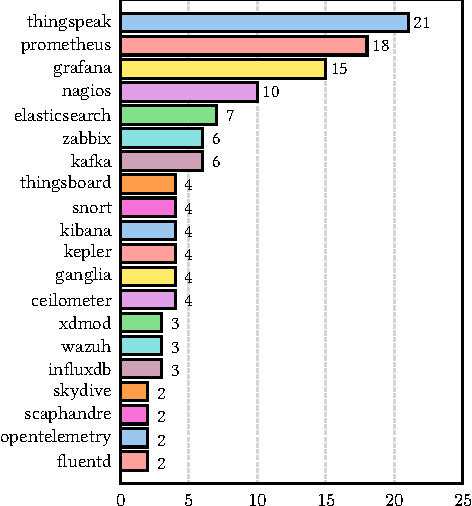
\includegraphics[width=0.85\linewidth]{assets/fig-tool-occurrence.pdf}
  \caption{Number of studies mentioning each tool (Tools appearing on a single study were omitted)}
  \Description[A bar chart showing how frequently each tool appears.]{Thingspeak appears first with 21 studies mentioning it; followed by prometheus with 18; grafana with 15; nagios with 10; elasticsearch with 7; zabbix and kafka with 6; thingsboard, snort, kibana, kepler, ganglia, ceilometer with 4; xdmod, wazuh, influxdb with 3; skydive, scaphandre, opentelemetry, fluentd with 2. All other tools that appear only on one study are omitted.}
  \label{fig-tool-occurrence}
\end{figure}

Figure~\ref{fig-tool-role} shows how frequent each role (as
defined in Section~\ref{selection-phase}) is. Some tools have
multiple roles (e.g. \emph{Grafana} has both \texttt{visualization} and
\texttt{alerting}). We can see a very high frequency in the collection
role; besides dedicated collectors, most instrumentation and processing
tools seem to have some sort of collection/aggregation mechanism
built-in.

\begin{figure}[!htbp]
  \centering
  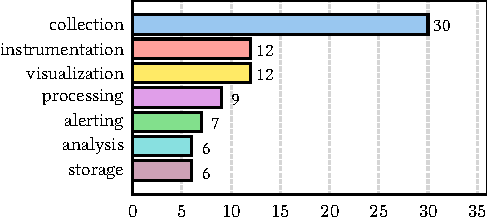
\includegraphics[width=0.85\linewidth]{assets/fig-tool-role.pdf}
  \caption{Number of tools per role (Some tools have multiple)}
  \Description[A bar chart showing which tool roles are more common.]{30 tools have collection role, 12 instrumentation, 12 visualization, 9 processing, 7 alerting, 6 analysis, and 6 storage.}
  \label{fig-tool-role}
\end{figure}

Figure~\ref{fig-yearly-distribution} shows the yearly
distribution of studies with at least one selected tool. We can see that
there is a growing trend, possibly indicating the increased interest in
the area. Our data contains studies from up until October 2025, thus
2024 studies are slightly more present than 2025 in the graph.

\begin{figure}[!htbp]
  \centering
  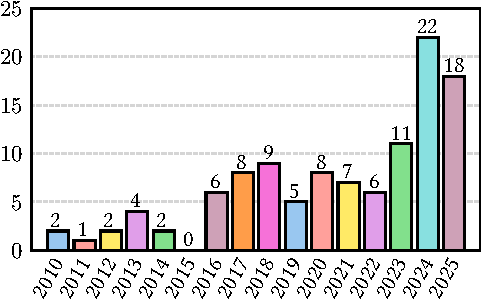
\includegraphics[width=0.85\linewidth]{assets/fig-yearly-distribution.pdf}
  \caption{Yearly study distribution}
  \Description[A column chart showing how many studies per year were selected.]{2010-2015 has few studies (1-4 per year), with the pace increasing in 2016-2023 (6-11), peaking in 2024-2025 with 22 and 18. The data collection was conducted in october 2025, explaining why 2025 is slightly lower than 2024.}
  \label{fig-yearly-distribution}
\end{figure}

\begin{framed}
Answering RQ1: \emph{Prometheus} is ubiquitous in the cloud
observability ecosystem. \emph{Nagios}, \emph{Grafana} and
\emph{ElasticSearch} are also frequent appearances. \emph{Thingspeak} is
an interesting outlier, representing the IoT sub-ecosystem. Collection
functionality is the most frequent, followed by instrumentation and
visualization.
\end{framed}

\subsection{Combinations of OSS Tools in Cloud Observability
Stacks}\label{combinations-of-oss-tools-in-cloud-observability-stacks}

To better visualize the relation data, we conducted a network analysis in
it, with the results shown in Figure~\ref{fig-relations}. For this figure,
we represent each tool as a node.

The graph edges are directed and weighted, serving as visualization of how
much a tool X relates to another tool Y. This is obtained, as described by
Section~\ref{analysis-phase}, through matching Y's name on X's codebase,
and represents relations such as integration features, comments mentioning
a borrowed snippet, documentation (usually comparing an alternative tool or
documenting integration), tests, and usage as libraries. As the codebase sizes
vary, the edge weights are normalized with the other edges originating from the
same node. Edges whose weights were lower than 0.05 (i.e. 5\% of all keyword
matches that codebase has) were hidden from the visualization, for improved
visibility.

The node size is derived from the sum of the weights of connections with that
node as destination, interpreted as how much important that the tool is to the
ecosystem. The node colors are a visualization of community clustering, that
groups tightly connected nodes together.

\begin{figure*}[!htbp]
  \centering
  \includesvg[keepaspectratio, width=0.95\linewidth]{assets/fig-relations.svg}
  \caption{Relations between tools, clustered and weighted by relative code occurrence}
  \Description[A directed graph of tools, their relations, centrality (visualized by size), and color coded based on community clustering.]{Some tools such as prometheus, elasticsearch, opentelemetry, and kafka are very well connected destinations (i.e. many other tools have mentions to it in their source code). Some common stacks are visible in the community clustering (e.g. influxdb, kapacitor, telegraf, have the same color, the same applies for elasticsearch, kibana, logstash, elastic beats.)}
  \label{fig-relations}
\end{figure*}

We can see in the figure how many tools relate to
\emph{Prometheus}; due to its format being the dominant one for metrics,
most other tools export metrics that are compatible with
\emph{Prometheus}. \emph{Thingspeak} is very disconnected from the other
tools, which hints that IoT tooling tends to be more standalone.
\emph{JoularJX} and \emph{Powerjoular}, a pair of tools built together
to, respectively, collect and aggregate power consumption data, also
appear isolated yet tightly coupled together. Some ecosystems can be
clearly seen being formed in the figure: the
\emph{ElasticSearch}+\emph{Logstash}+\emph{Kibana} ELK stack, and the
\emph{Telegraf}+\emph{InfluxDB}+\emph{Chronograf}+\emph{Kapacitor} TICK
stack being some obvious ones. The directionality of the relations is
also representative of how the tools behave, with \emph{Grafana} heavily
relating to \emph{Prometheus} (it has a \emph{Prometheus} datasource
built-in \cite{grafana-prometheus-docs}), but not the other way
around (i.e. \emph{Prometheus} knows almost nothing about
\emph{Grafana}).

\begin{framed}
Answering RQ2: some common stacks appear in this research, such as ELK
and TICK. Some tools are highly integrated in the ecosystem, with
\emph{Prometheus} being a central piece. \emph{Thingspeak} is an outlier
and shows that IoT tends toward standalone solutions.
\end{framed}

\section{Discussion}\label{discussion}

This section discusses our main findings, the threats to the validity of
this study, and future work.

\subsection{Main Findings}\label{main-findings}

The main findings resulting from our investigation of OSS tools for
cloud observability are:

\begin{itemize}
\item
  \textbf{Quantitative code matching can be a good proxy to find
  relations between codebases}. Our approach of matching the names of
  each tool on other tools' codebases worked.
  Figure~\ref{fig-relations} clearly shows clustering between
  well-known combinations: ElasticSearch+Logstash+Kibana (ELK stack),
  \emph{Telegraf}+\emph{InfluxDB}+\emph{Chronograf}+\emph{Kapacitor}
  (TICK stack). We can also see library usage (e.g.,
  \emph{OpenTelemetry}), the most ubiquitous tools (\emph{Prometheus})
  being highly referenced to, as well as some disconnected clusters
  (e.g., \emph{Powerjoular}+\emph{JoularJX}, \emph{Thingspeak}).
  Notably, our approach is very accurate in modeling directed relations,
  such as \emph{Grafana} integrating with \emph{Prometheus}
  \cite{grafana-prometheus-docs}, but not the other way around.
  Finally, our approach is heavily automated, and thus scales much
  better than the alternatives that involve manual labeling or more
  qualitative analysis. It should be interesting to apply these
  techniques to different Software Ecosystems.
\item
  \textbf{Some tools are de-facto standards, bringing interoperability
  but risking over-reliance}. It is interesting to see how
  \emph{Prometheus} has become so ubiquitous that there are references
  to it in the code of basically every single cloud observability tool
  that exists. If a software exports metrics, it is probably in the
  \emph{Prometheus} exposition format. Although \emph{Prometheus}'s
  community-based governance brings some safety, over-reliance on a
  single implementation can be problematic, thus bringing the need of
  standardization. \emph{OpenTelemetry} has recently emerged as a more
  standardized framework for different aspects of observability
  (including compatibility with the \emph{Prometheus} exposition format)
  \cite{prometheusotel}, and it is interesting to see adoption grow.
  The connection graph we built can be a helpful metric to determine
  which OSS tools are becoming critical, thus should be prioritized for
  standardization and/or alternative implementations by OSS communities
  and funding agencies.
\item
  \textbf{OSS and standardization can challenge proprietary lock-in}. Our data
  extraction step yielded some proprietary software (e.g. \emph{CloudWatch},
  \emph{AzureWatch}), most of them specific to a single cloud vendor.
  These were, however, often accompanied by OSS tools, a reminder that some
  of the OSS tools are so ubiquitous that vendors are effectively forced
  to implement support for them, further showing the strength OSS has in
  standardization and interoperability. Practitioners should consider
  prioritizing OSS when adopting observability tooling that needs to
  interoperate, for example, in multi-cloud scenarios.
\item
  \textbf{The line between an \emph{observability tool} and a tool that
  \emph{can be used for observability} can be thin}. During our manual
  selection step, some tools were difficult to classify. For example,
  \emph{Kafka} is not necessarily built for observability solutions, but
  its usage is so frequent that it becomes clear that it should be
  labeled as such. But what about other message queues? Or storage
  systems? Further research is required to effectively draw this line.
\end{itemize}

\subsection{Threats to Validity}\label{threats-to-validity}

As with any secondary studies, threats to validity must be considered as
well as mitigation actions, as discussed below:

\begin{itemize}
\item
  \textbf{Not all tools are mentioned in scientific literature}. There
  are a few tools the authors know about from their exposure to cloud
  observability solutions that did not appear in any of the abstracts
  our search yielded. This includes \emph{Mimir}, \emph{Loki},
  \emph{Graphite}, and \emph{Thanos}. This means that including other
  datasources and analysis techniques could provide a more complete set
  of tools. This is an acknowledged limitation in our study.
\item
  \textbf{Sparsity of dataset}. The abstract dataset is very sparse,
  making validation harder. Only \textbf{4\%} of the total corpus
  includes at least one tool from the final selection. We mitigated this
  by building a validation set that included both known tools as well as
  randomly sampled studies.
\item
  \textbf{LLM bias}. Although we calibrated the prompt to minimize false
  negatives, the LLM can be biased towards more well-known tools. We mitigated
  this by inspecting the abstracts of all 774 extracted studies (i.e. studies
  from which the LLM extracted at least one tool), this same inspection is,
  however, not possible in the negative population, as it is very large. The
  mitigation provided by the validation set (Section~\ref{validation-set}), with
  a high recall value, is considered sufficient.
\item
  \textbf{Abstracts may not contain every tool relevant to the work}.
  Using only the abstracts (as opposed to the fulltexts) can leave out
  relevant tools. This is somewhat mitigated by the large corpus of
  studies we used, and is a tradeoff we accepted to build a more
  automated research method.
\item
  \textbf{Code matches can contain false positives}. Some codebases,
  such as ElasticSearch's, contain files such as wordlists. This is
  mitigated by making the weights relative and discarding less relevant
  edges. Future research could involve additional heuristics.
\item
  \textbf{Code matches can contain transitive relations}. Transitive
  dependencies/integrations are also frequently matched, which might be
  an issue if the intention is to only model direct ones. This can be
  partially mitigated by excluding lockfiles. We decided to not
  qualitatively differentiate the nature of each relation, so this is
  considered out of scope for this paper.
\item
  \textbf{Human error during selection}. As with any classification
  based on human decisions, our selection process could contain errors
  or be biased. This was mitigated by consensus between the authors and
  by carefully researching each candidate tool.
\end{itemize}

\subsection{Future Work}\label{future-work}

Based on the results of our investigation, we can suggest the following
future work:

\begin{itemize}
\item
  \textbf{Qualitative analysis on the relations}. Our approach with the
  relations between tools was very quantitative, with no regard for the nature of
  the code nor any attempt to filter false positive matches. By conducting a more
  qualitative analysis of each individual relation identified, one could gain a
  better understanding of the relation between tools, and how good of a proxy the
  quantitative analysis is.
\item
  \textbf{Other datasources besides academic studies}. Although useful
  for casting a wide net, academic studies might not be enough to locate
  all tooling, specially emerging ones. Other methods such a multivocal
  literature reviews to find the set of tools might be interesting to
  explore.
\item
  \textbf{Applying our method to other ecosystems}. The code keyword
  matching approach is simple, very scalable, and seems to provide good
  results. One could apply this technique to other ecosystems.
\item
  \textbf{A better definition of observability tooling is needed}. Some
  tools are used in observability but do not define themselves as
  observability tools. Some better heuristic to make this classification
  could be explored.
\item
  \textbf{Other heuristics for finding relations}. Research on more
  heuristics for the relations can be interesting. For example, by
  analyzing the common contributors between two projects, one could
  measure integration and/or cross-pollination between different
  software projects.
\end{itemize}

\section{Conclusions}\label{conclusions}

As IT operations shift into an Engineering activity, Observability also
grows as an important topic for SE research. In our work, our objective
was to provide an accurate starting point to researchers exploring the
OSS Observability ecosystem. Our research shows a selection of 45 OSS
tools, a categorization on their functionality, and a quantitative
measure of the relations between one other. A few tools are shown to
have a central role in the ecosystem, such as \emph{Prometheus}, others
appear clustered in stacks, such as \emph{ELK} (\emph{ElasticSearch},
\emph{Logstash}, \emph{Kibana}) and TICK (\emph{Telegraf}),
\emph{InfluxDB}, \emph{Chronograf}, \emph{Kapacitor}). We also showcase
some outliers, such as \emph{Thingspeak} which does not relate to any
other tool we have researched, as well as tools that appear isolated as
a pair, such as \emph{JoularJX} and \emph{PowerJoular}.

Our methodology is very automated and can be helpful for any exploratory
study of a Software Ecosystem where source code is available for
analysis. This sort of overview can be helpful for practitioners to
locate additional components their observability stack might be missing,
as well as to discover alternatives for tools they are using.

\begin{acks}

This study was financed by FAPESP (2023/00488-5), CNPq (313245/2021-5),
CAPES (001), and by ITEA4 and RVO under grant agreement No.~22035 MAST
(\url{https://itea4.org/project/mast.html}).

\end{acks}

\bibliographystyle{ACM-Reference-Format}
\bibliography{references}

\appendix

\onecolumn
\section{Selected Tools}
\begin{table*}[!htbp]
  \caption{Selected Tools}
  \label{table-selected-tools}
  \centering

  \begin{tabular}{c c c}
  \hline
  \textbf{Tool} & \textbf{Studies} & \textbf{Roles} \\
  \hline
  thingspeak & 21 & collection, storage \\
  prometheus & 18 & instrumentation, collection, alerting \\
  grafana & 15 & visualization, alerting \\
  nagios & 10 & collection, alerting \\
  elasticsearch & 7 & storage \\
  kafka & 6 & processing \\
  zabbix & 6 & collection, alerting, visualization \\
  ceilometer & 4 & collection \\
  ganglia & 4 & collection, processing, visualization \\
  kepler & 4 & instrumentation \\
  kibana & 4 & visualization \\
  snort & 4 & collection \\
  thingsboard & 4 & collection, processing, visualization, analysis \\
  influxdb & 3 & storage, processing \\
  wazuh & 3 & instrumentation, alerting, visualization, collection,
  analysis \\
  xdmod & 3 & instrumentation, collection, analysis \\
  fluentd & 2 & collection \\
  opentelemetry & 2 & instrumentation, collection \\
  scaphandre & 2 & instrumentation, collection \\
  skydive & 2 & collection \\
  cacti & 1 & collection, visualization \\
  cadvisor & 1 & collection \\
  chronograf & 1 & visualization \\
  collectd & 1 & instrumentation, collection \\
  collectl & 1 & collection \\
  elastic beats & 1 & instrumentation \\
  flume & 1 & collection, processing \\
  jaeger & 1 & collection, visualization \\
  joularjx & 1 & instrumentation, collection \\
  kapacitor & 1 & processing, alerting \\
  logstash & 1 & collection, processing \\
  monasca & 1 & storage, processing \\
  netdata & 1 & collection, alerting \\
  net-snmp & 1 & collection \\
  ntopng & 1 & instrumentation, collection \\
  opentsdb & 1 & storage \\
  powerjoular & 1 & collection \\
  sysdig & 1 & instrumentation \\
  syslog-ng & 1 & collection \\
  systemtap & 1 & instrumentation \\
  telegraf & 1 & processing, collection \\
  tetragon & 1 & collection, analysis \\
  tracecompass & 1 & visualization, analysis \\
  zenoss & 1 & collection, visualization \\
  zipkin & 1 & storage, visualization, analysis \\
  \hline
  \end{tabular}
  \smallskip
\end{table*}

\end{document}
